\documentclass[tikz,border=2pt]{standalone}
\usepackage[T1]{fontenc}
\usepackage[scaled=0.95]{helvet}
\renewcommand{\familydefault}{\sfdefault}
\usetikzlibrary{arrows.meta}
% Chapter dependency map in the flat stack-diagram style (muted accent blocks, white
% bold type). Coordinates follow the original SVG; edges are unchanged from it.
\definecolor{accent}{HTML}{1F407A}
\colorlet{stackfill}{accent!60!white}
\colorlet{bandfill}{accent!8!white}
\definecolor{ink}{RGB}{38,38,42}
\definecolor{softink}{RGB}{105,105,110}
\definecolor{lightlink}{RGB}{120,130,145}
\begin{document}
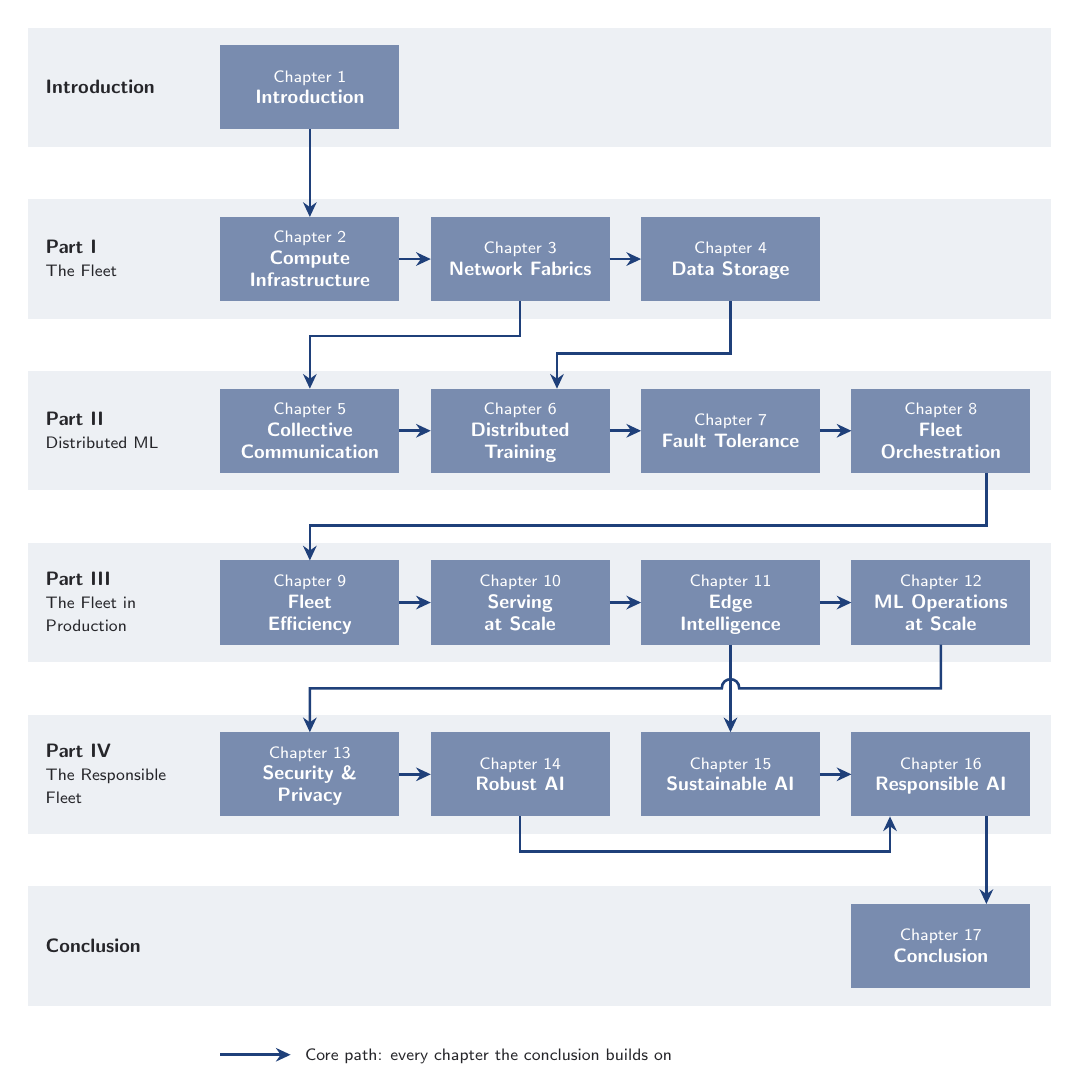
\begin{tikzpicture}[x=1pt,y=-1pt]

\fill[bandfill] (5.07,5.07) rectangle (374.93,48.13);
\fill[bandfill] (5.07,67.13) rectangle (374.93,110.20);
\fill[bandfill] (5.07,129.20) rectangle (374.93,172.27);
\fill[bandfill] (5.07,191.27) rectangle (374.93,234.33);
\fill[bandfill] (5.07,253.33) rectangle (374.93,296.40);
\fill[bandfill] (5.07,315.40) rectangle (374.93,358.47);
\fill[stackfill] (74.73,11.40) rectangle (139.33,41.80);
\fill[stackfill] (74.73,73.47) rectangle (139.33,103.87);
\fill[stackfill] (150.73,73.47) rectangle (215.33,103.87);
\fill[stackfill] (226.73,73.47) rectangle (291.33,103.87);
\fill[stackfill] (74.73,135.53) rectangle (139.33,165.93);
\fill[stackfill] (150.73,135.53) rectangle (215.33,165.93);
\fill[stackfill] (226.73,135.53) rectangle (291.33,165.93);
\fill[stackfill] (302.73,135.53) rectangle (367.33,165.93);
\fill[stackfill] (74.73,197.60) rectangle (139.33,228.00);
\fill[stackfill] (150.73,197.60) rectangle (215.33,228.00);
\fill[stackfill] (226.73,197.60) rectangle (291.33,228.00);
\fill[stackfill] (302.73,197.60) rectangle (367.33,228.00);
\fill[stackfill] (74.73,259.67) rectangle (139.33,290.07);
\fill[stackfill] (150.73,259.67) rectangle (215.33,290.07);
\fill[stackfill] (226.73,259.67) rectangle (291.33,290.07);
\fill[stackfill] (302.73,259.67) rectangle (367.33,290.07);
\fill[stackfill] (302.73,321.73) rectangle (367.33,352.13);
\node[anchor=base west,inner sep=0pt,text=ink,font=\bfseries\fontsize{7.0}{8.0}\selectfont] at (11.40,28.82) {Introduction};
\node[anchor=base west,inner sep=0pt,text=ink,font=\bfseries\fontsize{7.0}{8.0}\selectfont] at (11.40,86.77) {Part I};
\node[anchor=base west,inner sep=0pt,text=ink,font=\fontsize{6.3}{7.3}\selectfont] at (11.40,95.00) {The Fleet};
\node[anchor=base west,inner sep=0pt,text=ink,font=\bfseries\fontsize{7.0}{8.0}\selectfont] at (11.40,148.83) {Part II};
\node[anchor=base west,inner sep=0pt,text=ink,font=\fontsize{6.3}{7.3}\selectfont] at (11.40,157.07) {Distributed ML};
\node[anchor=base west,inner sep=0pt,text=ink,font=\bfseries\fontsize{7.0}{8.0}\selectfont] at (11.40,206.78) {Part III};
\node[anchor=base west,inner sep=0pt,text=ink,font=\fontsize{6.3}{7.3}\selectfont] at (11.40,215.02) {The Fleet in};
\node[anchor=base west,inner sep=0pt,text=ink,font=\fontsize{6.3}{7.3}\selectfont] at (11.40,223.25) {Production};
\node[anchor=base west,inner sep=0pt,text=ink,font=\bfseries\fontsize{7.0}{8.0}\selectfont] at (11.40,268.85) {Part IV};
\node[anchor=base west,inner sep=0pt,text=ink,font=\fontsize{6.3}{7.3}\selectfont] at (11.40,277.08) {The Responsible};
\node[anchor=base west,inner sep=0pt,text=ink,font=\fontsize{6.3}{7.3}\selectfont] at (11.40,285.32) {Fleet};
\node[anchor=base west,inner sep=0pt,text=ink,font=\bfseries\fontsize{7.0}{8.0}\selectfont] at (11.40,339.15) {Conclusion};
\node[anchor=base,inner sep=0pt,text=white,font=\fontsize{6.3}{7.3}\selectfont] at (107.03,24.70) {Chapter 1};
\node[anchor=base,inner sep=0pt,text=white,font=\bfseries\fontsize{6.6}{7.6}\selectfont] at (107.03,32.62) {Introduction};
\node[anchor=base,inner sep=0pt,text=white,font=\fontsize{6.3}{7.3}\selectfont] at (107.03,82.84) {Chapter 2};
\node[anchor=base,inner sep=0pt,text=white,font=\bfseries\fontsize{6.6}{7.6}\selectfont] at (107.03,90.69) {Compute};
\node[anchor=base,inner sep=0pt,text=white,font=\bfseries\fontsize{6.6}{7.6}\selectfont] at (107.03,98.67) {Infrastructure};
\node[anchor=base,inner sep=0pt,text=white,font=\fontsize{6.3}{7.3}\selectfont] at (183.03,86.77) {Chapter 3};
\node[anchor=base,inner sep=0pt,text=white,font=\bfseries\fontsize{6.6}{7.6}\selectfont] at (183.03,94.68) {Network Fabrics};
\node[anchor=base,inner sep=0pt,text=white,font=\fontsize{6.3}{7.3}\selectfont] at (259.03,86.77) {Chapter 4};
\node[anchor=base,inner sep=0pt,text=white,font=\bfseries\fontsize{6.6}{7.6}\selectfont] at (259.03,94.68) {Data Storage};
\node[anchor=base,inner sep=0pt,text=white,font=\fontsize{6.3}{7.3}\selectfont] at (107.03,144.91) {Chapter 5};
\node[anchor=base,inner sep=0pt,text=white,font=\bfseries\fontsize{6.6}{7.6}\selectfont] at (107.03,152.76) {Collective};
\node[anchor=base,inner sep=0pt,text=white,font=\bfseries\fontsize{6.6}{7.6}\selectfont] at (107.03,160.74) {Communication};
\node[anchor=base,inner sep=0pt,text=white,font=\fontsize{6.3}{7.3}\selectfont] at (183.03,144.91) {Chapter 6};
\node[anchor=base,inner sep=0pt,text=white,font=\bfseries\fontsize{6.6}{7.6}\selectfont] at (183.03,152.76) {Distributed};
\node[anchor=base,inner sep=0pt,text=white,font=\bfseries\fontsize{6.6}{7.6}\selectfont] at (183.03,160.74) {Training};
\node[anchor=base,inner sep=0pt,text=white,font=\fontsize{6.3}{7.3}\selectfont] at (259.03,148.83) {Chapter 7};
\node[anchor=base,inner sep=0pt,text=white,font=\bfseries\fontsize{6.6}{7.6}\selectfont] at (259.03,156.75) {Fault Tolerance};
\node[anchor=base,inner sep=0pt,text=white,font=\fontsize{6.3}{7.3}\selectfont] at (335.03,144.91) {Chapter 8};
\node[anchor=base,inner sep=0pt,text=white,font=\bfseries\fontsize{6.6}{7.6}\selectfont] at (335.03,152.76) {Fleet};
\node[anchor=base,inner sep=0pt,text=white,font=\bfseries\fontsize{6.6}{7.6}\selectfont] at (335.03,160.74) {Orchestration};
\node[anchor=base,inner sep=0pt,text=white,font=\fontsize{6.3}{7.3}\selectfont] at (107.03,206.97) {Chapter 9};
\node[anchor=base,inner sep=0pt,text=white,font=\bfseries\fontsize{6.6}{7.6}\selectfont] at (107.03,214.83) {Fleet};
\node[anchor=base,inner sep=0pt,text=white,font=\bfseries\fontsize{6.6}{7.6}\selectfont] at (107.03,222.81) {Efficiency};
\node[anchor=base,inner sep=0pt,text=white,font=\fontsize{6.3}{7.3}\selectfont] at (183.03,206.97) {Chapter 10};
\node[anchor=base,inner sep=0pt,text=white,font=\bfseries\fontsize{6.6}{7.6}\selectfont] at (183.03,214.83) {Serving};
\node[anchor=base,inner sep=0pt,text=white,font=\bfseries\fontsize{6.6}{7.6}\selectfont] at (183.03,222.81) {at Scale};
\node[anchor=base,inner sep=0pt,text=white,font=\fontsize{6.3}{7.3}\selectfont] at (259.03,206.97) {Chapter 11};
\node[anchor=base,inner sep=0pt,text=white,font=\bfseries\fontsize{6.6}{7.6}\selectfont] at (259.03,214.83) {Edge};
\node[anchor=base,inner sep=0pt,text=white,font=\bfseries\fontsize{6.6}{7.6}\selectfont] at (259.03,222.81) {Intelligence};
\node[anchor=base,inner sep=0pt,text=white,font=\fontsize{6.3}{7.3}\selectfont] at (335.03,206.97) {Chapter 12};
\node[anchor=base,inner sep=0pt,text=white,font=\bfseries\fontsize{6.6}{7.6}\selectfont] at (335.03,214.83) {ML Operations};
\node[anchor=base,inner sep=0pt,text=white,font=\bfseries\fontsize{6.6}{7.6}\selectfont] at (335.03,222.81) {at Scale};
\node[anchor=base,inner sep=0pt,text=white,font=\fontsize{6.3}{7.3}\selectfont] at (107.03,269.04) {Chapter 13};
\node[anchor=base,inner sep=0pt,text=white,font=\bfseries\fontsize{6.6}{7.6}\selectfont] at (107.03,276.89) {Security \&};
\node[anchor=base,inner sep=0pt,text=white,font=\bfseries\fontsize{6.6}{7.6}\selectfont] at (107.03,284.87) {Privacy};
\node[anchor=base,inner sep=0pt,text=white,font=\fontsize{6.3}{7.3}\selectfont] at (183.03,272.97) {Chapter 14};
\node[anchor=base,inner sep=0pt,text=white,font=\bfseries\fontsize{6.6}{7.6}\selectfont] at (183.03,280.88) {Robust AI};
\node[anchor=base,inner sep=0pt,text=white,font=\fontsize{6.3}{7.3}\selectfont] at (259.03,272.97) {Chapter 15};
\node[anchor=base,inner sep=0pt,text=white,font=\bfseries\fontsize{6.6}{7.6}\selectfont] at (259.03,280.88) {Sustainable AI};
\node[anchor=base,inner sep=0pt,text=white,font=\fontsize{6.3}{7.3}\selectfont] at (335.03,272.97) {Chapter 16};
\node[anchor=base,inner sep=0pt,text=white,font=\bfseries\fontsize{6.6}{7.6}\selectfont] at (335.03,280.88) {Responsible AI};
\node[anchor=base,inner sep=0pt,text=white,font=\fontsize{6.3}{7.3}\selectfont] at (335.03,335.03) {Chapter 17};
\node[anchor=base,inner sep=0pt,text=white,font=\bfseries\fontsize{6.6}{7.6}\selectfont] at (335.03,342.95) {Conclusion};
\node[anchor=base west,inner sep=0pt,text=ink,font=\fontsize{6.3}{7.3}\selectfont] at (105.13,378.42) {Core path: every chapter the conclusion builds on};
\draw[accent,line width=0.95pt,-{Stealth[length=5.3pt,width=4.9pt]}] (107.03,41.80) -- (107.03,73.47);
\draw[accent,line width=0.95pt,-{Stealth[length=5.3pt,width=4.9pt]}] (139.33,88.67) -- (150.73,88.67);
\draw[accent,line width=0.95pt,-{Stealth[length=5.3pt,width=4.9pt]}] (215.33,88.67) -- (226.73,88.67);
\draw[accent,line width=0.95pt,-{Stealth[length=5.3pt,width=4.9pt]}] (183.03,103.87) -- (183.03,116.53) -- (107.03,116.53) -- (107.03,135.53);
\draw[accent,line width=0.95pt,-{Stealth[length=5.3pt,width=4.9pt]}] (215.33,150.73) -- (226.73,150.73);
\draw[accent,line width=0.95pt,-{Stealth[length=5.3pt,width=4.9pt]}] (259.03,103.87) -- (259.03,122.87) -- (196.33,122.87) -- (196.33,135.53);
\draw[accent,line width=0.95pt,-{Stealth[length=5.3pt,width=4.9pt]}] (139.33,150.73) -- (150.73,150.73);
\draw[accent,line width=0.95pt,-{Stealth[length=5.3pt,width=4.9pt]}] (291.33,150.73) -- (302.73,150.73);
\draw[accent,line width=0.95pt,-{Stealth[length=5.3pt,width=4.9pt]}] (351.50,165.93) -- (351.50,184.93) -- (107.03,184.93) -- (107.03,197.60);
\draw[accent,line width=0.95pt,-{Stealth[length=5.3pt,width=4.9pt]}] (139.33,212.80) -- (150.73,212.80);
\draw[accent,line width=0.95pt,-{Stealth[length=5.3pt,width=4.9pt]}] (215.33,212.80) -- (226.73,212.80);
\draw[accent,line width=0.95pt,-{Stealth[length=5.3pt,width=4.9pt]}] (291.33,212.80) -- (302.73,212.80);
\draw[accent,line width=0.95pt,-{Stealth[length=5.3pt,width=4.9pt]}] (259.03,228.00) -- (259.03,259.67);
\draw[accent,line width=0.95pt,-{Stealth[length=5.3pt,width=4.9pt]}] (335.03,228.00) -- (335.03,243.83) -- (262.20,243.83) .. controls (262.20,239.40) and (255.87,239.40) .. (255.87,243.83) -- (107.03,243.83) -- (107.03,259.67);
\draw[accent,line width=0.95pt,-{Stealth[length=5.3pt,width=4.9pt]}] (139.33,274.87) -- (150.73,274.87);
\draw[accent,line width=0.95pt,-{Stealth[length=5.3pt,width=4.9pt]}] (291.33,274.87) -- (302.73,274.87);
\draw[accent,line width=0.95pt,-{Stealth[length=5.3pt,width=4.9pt]}] (183.03,290.07) -- (183.03,302.73) -- (316.67,302.73) -- (316.67,290.07);
\draw[accent,line width=0.95pt,-{Stealth[length=5.3pt,width=4.9pt]}] (351.50,290.07) -- (351.50,321.73);
\draw[accent,line width=0.95pt,-{Stealth[length=5.3pt,width=4.9pt]}] (74.73,376.20) -- (100.07,376.20);
\end{tikzpicture}
\end{document}
